

\documentclass[paper=a4, fontsize=11pt,twoside]{scrartcl}	% KOMA

\usepackage[a4paper,pdftex]{geometry}	% A4paper margins
\setlength{\oddsidemargin}{5mm}			% Remove 'twosided' indentation
\setlength{\evensidemargin}{5mm}

% \usepackage[english]{babel}
\usepackage[protrusion=true,expansion=true]{microtype}	
\usepackage{amsmath,amsfonts,amsthm,amssymb}
\usepackage{graphicx}
\usepackage[spanish]{babel}
\usepackage[hidelinks]{hyperref}
\usepackage{graphicx}
\usepackage{xcolor}
\usepackage{fancyhdr}
\usepackage{hyperref}
\newcommand{\HRule}[1]{\rule{\linewidth}{#1}} 	% Horizontal rule
\usepackage{float}

\makeatletter							% Title
\def\printtitle{%						
    {\centering \@title\par}}
\makeatother									

\makeatletter							% Author
\def\printauthor{%					
    {\centering \large \@author}}				
\makeatother							

\title{	\normalsize \textsc{ANEXO DE DISEÑO DE HARDWARE} 	% Subtitle
		 	\\[2.0cm]								% 2cm spacing
			\HRule{0.5pt} \\						% Upper rule
			\LARGE \textbf{\uppercase{Sistemas de posicionamiento de objetos mediante la tecnología Bluetooth Low Energy, modo Beacon}}	% Title
			\HRule{2pt} \\ [0.5cm]		% Lower rule + 0.5cm spacing
			\normalsize \today			% Todays date
		}
\author{
		Rubén Arce Domingo\\	
		Máster en automatización y robótica\\	
        industrial\\
        akimbo170@gmail.com \\
        % \texttt{akimbo170@gmail.com} \\
}
\begin{document}
\thispagestyle{empty}		% Remove page numbering on this page
\printtitle					% Print the title data as defined above
  	\vfill
\printauthor				% Print the author data as defined above
\newpage

% \title{Anexo desarrollo de hardware}

% \author{Rubén Arce}
% \date{\today}
% \maketitle
\cleardoublepage
\tableofcontents
\listoffigures
\cleardoublepage
\pagestyle{fancy}
\fancyfoot[R]{Rubén Arce}
\fancyfoot[L]{BLE Tracking - 2020}

\section{Introducción}
    Los diseños eléctricos y el trazado de las pistas del circuito se han llevado a cabo con Kicad en 
    su versión 5.1.6. Se ha empleado este programa debido a que, en primer lugar es de software libre y
    completamente gratuito y, en segundo lugar, debido a que puede funcionar en Linux. Además de que es capaz de llevar a cabo 
    cualquier diseño profesional sin problema de licencias o versiones incompatibles.

    Por otro lado, todas las PCBs se han fabricado en dos capas con un espesor estándar de 1,6mm y con acabado superficial
    HASH plomo estaño en los primeros prototipos. En la versión final se empleará el acabado ENIG, o de oro 
    electrolítico, para mejorar las especificaciones y durabilidad de la misma.

    Por último mencionar que se han empleado tanto componentes SMD como through hole y se ha priorizado el precio en la selección de los mismos.
\section{Emisor Beacon}
    \subsection{Aspectos a considerar}
        Las premisas para seleccionar el mejor microcontrolador han sido las siguientes: 
        \begin{enumerate}
            \item Bajo consumo.
            \item Tamaño reducido.
            \item Bluetooth y posibilidad de wifi en caso de eliminar el dispositivo emisor.
            \item Precio muy competitivo.
        \end{enumerate}
    \subsection{Circuito eléctrico}
        \subsubsection{Microcontrolador} 
            En el caso del microcontrolador, se ha optado por un ESP32 de la empresa Espressif (\url{https://www.espressif.com/})
            debido en gran medida a que dispone de wifi y bluetooth, así como de unas excelentes herramientas
            de desarrollo de software. 
        \subsubsection{Alimentación} 
            Para llevar a cabo la alimentación del microcontrolador y, teniendo en cuenta que se han de garantizar los 3,3V en la entrada
            del micro, se ha optado por una batería de Ion-Litio de 1400mAh que además tiene un tamaño reducido. El rango de tensión de la
            tarjeta va de 12V a 3,6V en el caso de que se opte por otro método de alimentación.
    \subsection{PCB de control}
        \paragraph{}
        Una vez tenidas en cuenta estas especificaciones, en el esquema eléctrico se ha llevado a cabo el ruteo de la tarjeta.
        Vemos que se ha elaborado el trazado de pistas con planos de masa para prevenir interferencias electromagnéticas
        y conseguir que no afecte demasiado a la electrónica. En las diguras 1 y 2 podemos ver imágenes de los renderizados y circuitos 
        eléctricos.
        \begin{center}
            \begin{figure}[H]
                \centering
                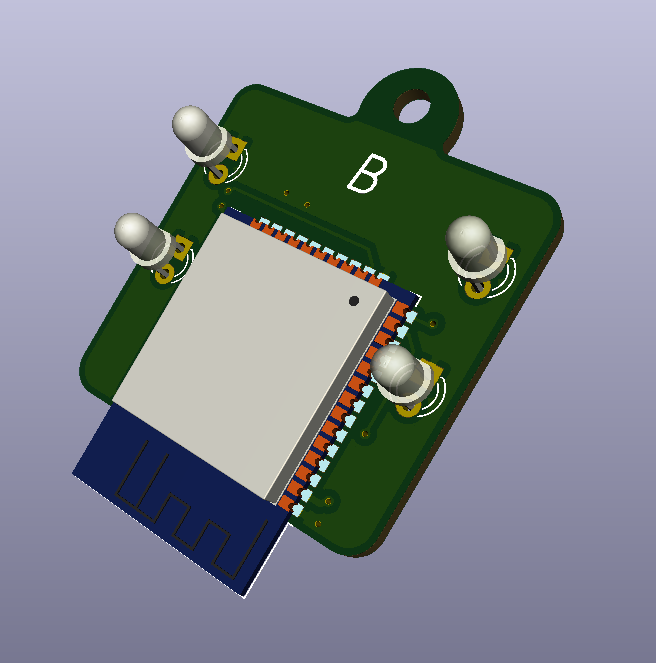
\includegraphics[width=0.4\textwidth]{../emiter_1.PNG}
                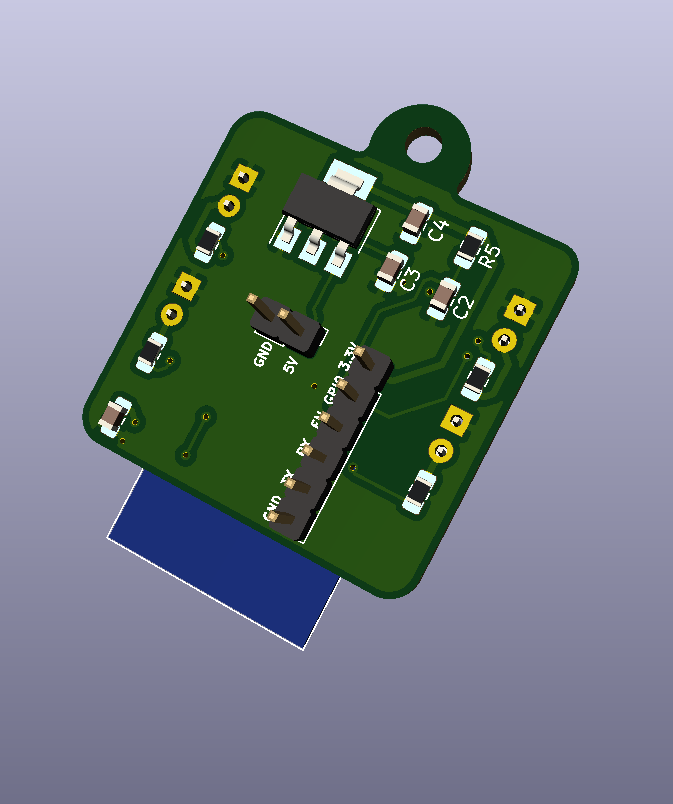
\includegraphics[width=0.35\textwidth]{../emiter_2.PNG}
                \caption{Renderizado de PCB del Beacon.}
                \label{fig:mesh8}
            \end{figure}    
        \end{center}
        \begin{center}
            \begin{figure}[H]
                \centering
                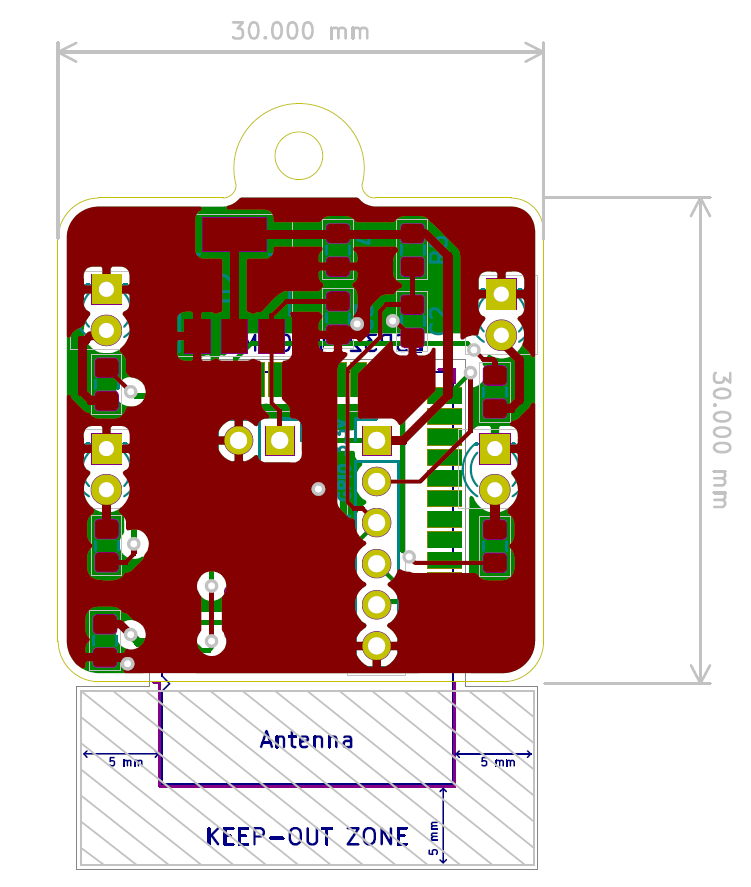
\includegraphics[width=0.40\textwidth]{../emiter_PCB.PNG}
                \caption{PCB del Beacon obtenida con Kicad.}
                \label{fig:mesh9}
            \end{figure}    
        \end{center}
        Se ha dejado la zona de la antena despejada para mejor la ganancia de la misma y en consecuencia el alcance, en el caso 
        del Beacon se usarán las antenas que integra el microcontrolador.
    \subsection{Imágenes reales}
        \paragraph{}
        Tras llevar a cabo la fabricación de las tarjetas prototipo podemos ver los resultados en la figura 3.
        \begin{center}
            \begin{figure}[ht]
                \centering
                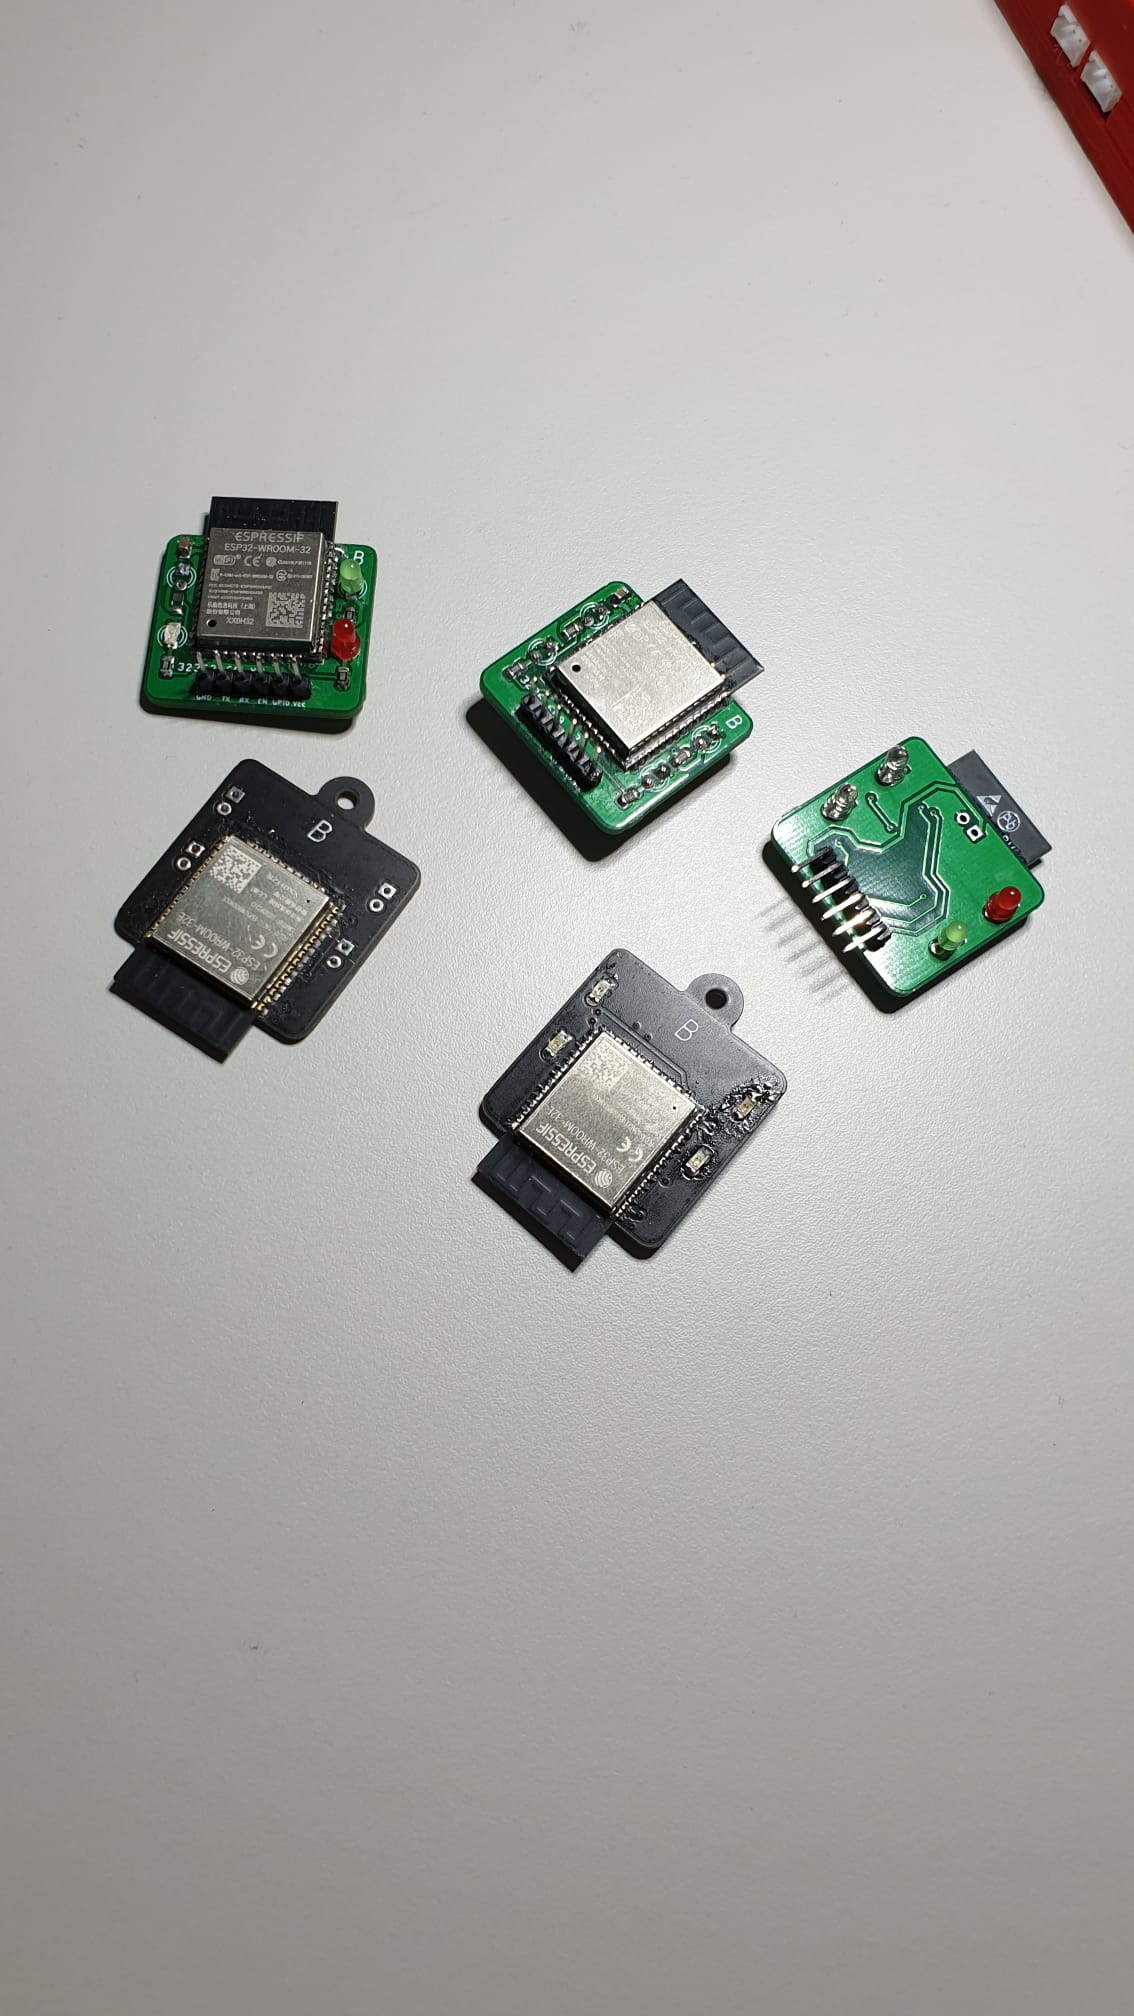
\includegraphics[width=0.5\textwidth]{../real_beacon_pcb.jpeg}
                \caption{PCB real fabricada y soldada}
                \label{fig:mesh3}
            \end{figure}    
        \end{center}       
\section{Receptor Beacon o gateway}
    \subsection{Aspectos a considerar}
        \begin{enumerate}
            \item Velocidad de procesamiento: El número máximo de equipos a localizar puede ser superior a 500, es por ello 
            por lo que quedan descartados los microcontrodores de 8 bits y cristales de menos de 16MHz.
            \item Wifi/bluetooth: Ha de escuchar a los Beacons y subir los datos a internet, es por ello por lo que se hace 
            indispesable que cuente con hardware que permita las dos acciones.
        \end{enumerate}

    \subsection{Circuito eléctrico}
        \subsubsection{Microcontrolador} 
            Teniendo en cuenta estas condiciones previas y contando con procesadores ESP32 del diseño anterior, se ha optado por compartir 
            el procesador para ambos equipos. Con esto conseguimos que el software y librerías sean compatibles al 100\% y se ahorre tiempo
            de desarrollo.
        \subsubsection{Alimentación} 
            En este caso puesto que la tarjeta se encontrará estática en un lugar cercano a un enchufe se brindan las siguientes opciones
            de alimentación:
            \begin{enumerate}
                \item 220 VAC.
                \item 12 VDC.
                \item 5 VDC, en el caso de que se disponga de un ordenador cerca se podría conectar por USB.
            \end{enumerate}
            En la figura 4 podemos ver el circuito responsable, mediante un jumper. Se facilita el cambio de alimentación para las distintas necesidades 
            de los clientes.
            \begin{center}
                \begin{figure}[h]
                    \centering
                    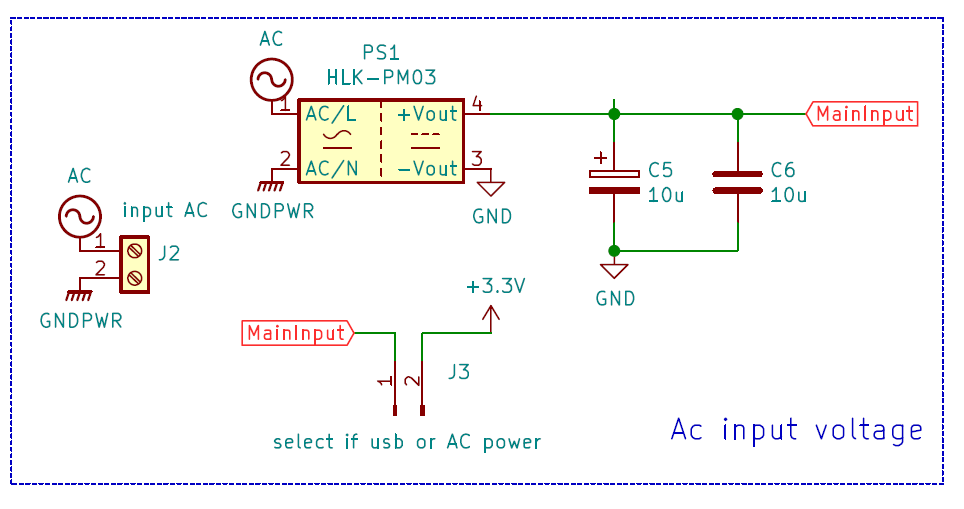
\includegraphics[width=0.8\textwidth]{../receiver_main_power.PNG}
                    \caption{Fuentes de alimentación de la PCB master.}
                    \label{fig:mesh4}
                \end{figure}    
            \end{center}    
    \subsection{PCB de control}
        Se ha optado por llevar a cabo el trazado de pistas de alimentación por la cara top y las de señal por la bottom, vemos que hay dos 
        conectores en los extremos de la tarjeta, uno con una UART para comunicarse con otros sistemas de la planta y otro conector para sensores
        i2c, pensado para la lectura de humedad y temperatura, así como para el envío de estos datos a la web de control. En la figura 5 se aprecia 
        con mayor detalle la PCB del master en un renderizado obtenido con Kicad.

        En el apartado de planos se puede ver con mayor detalle el esquema eléctrico y dimensiones de la tarjeta. 
        \begin{center}
            \begin{figure}[ht]
                \centering
                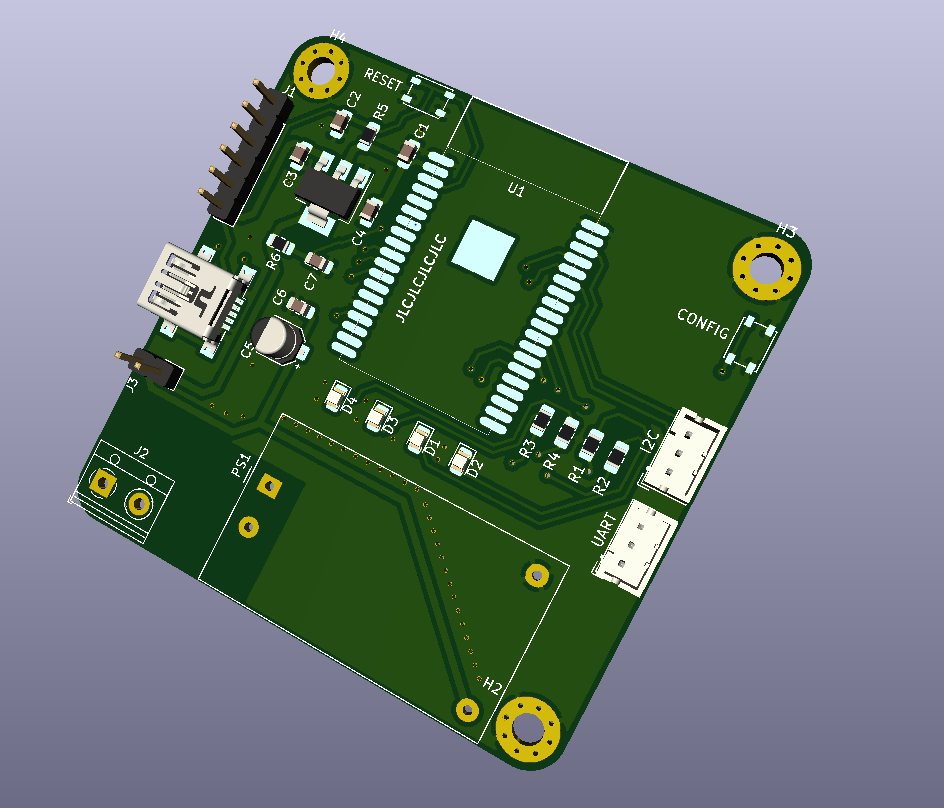
\includegraphics[width=0.4\textwidth]{../receiver_1.PNG}
                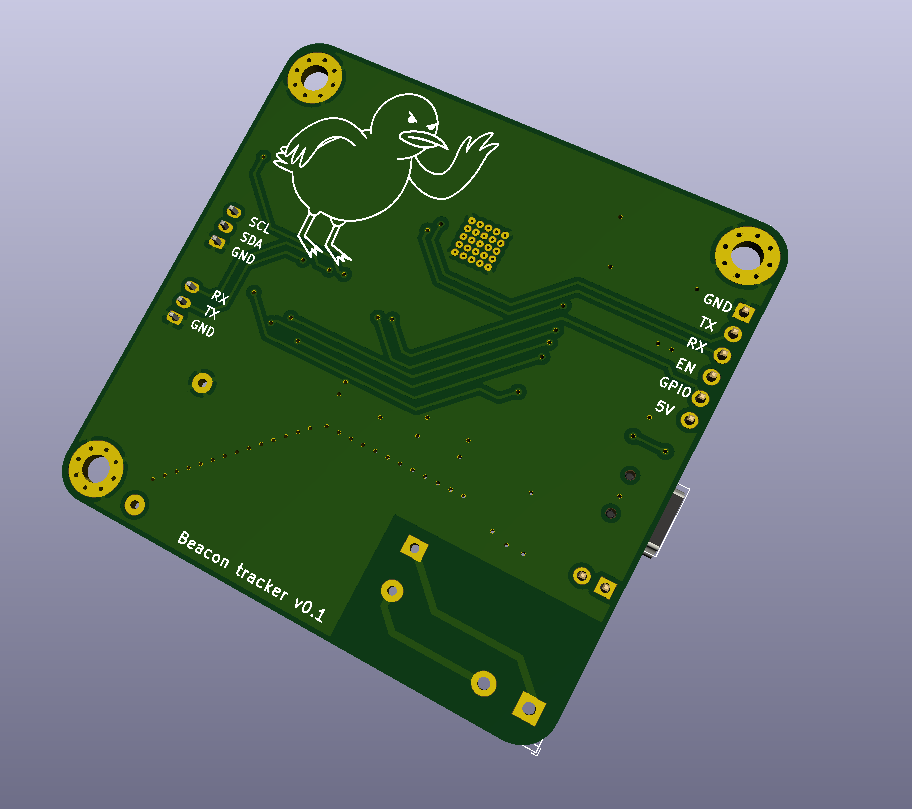
\includegraphics[width=0.4\textwidth]{../receiver_2.PNG}
                \caption{Renderizado de PCB del master o gateway.}
                \label{fig:mesh5}
            \end{figure}    
        \end{center}
        \begin{center}
            \begin{figure}[ht]
                \centering
                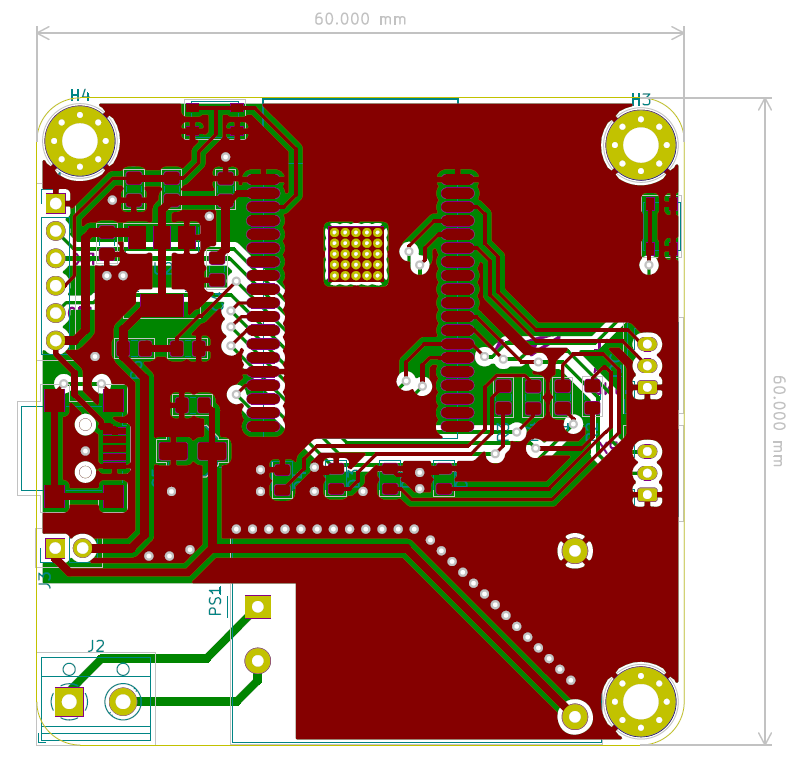
\includegraphics[width=0.5\textwidth]{../receiver_PCB.PNG}
                \caption{Renderizado de PCB del master o gateway.}
                \label{fig:mesh6}
            \end{figure}    
        \end{center}
    \subsection{Imágenes reales}
        Por último y tras fabricar las tarjetas e imprimir las cajas que lo contienen se obtiene el resultado de las figuras 6 y 7.
        \begin{center}
            \begin{figure}[ht]
                \centering
                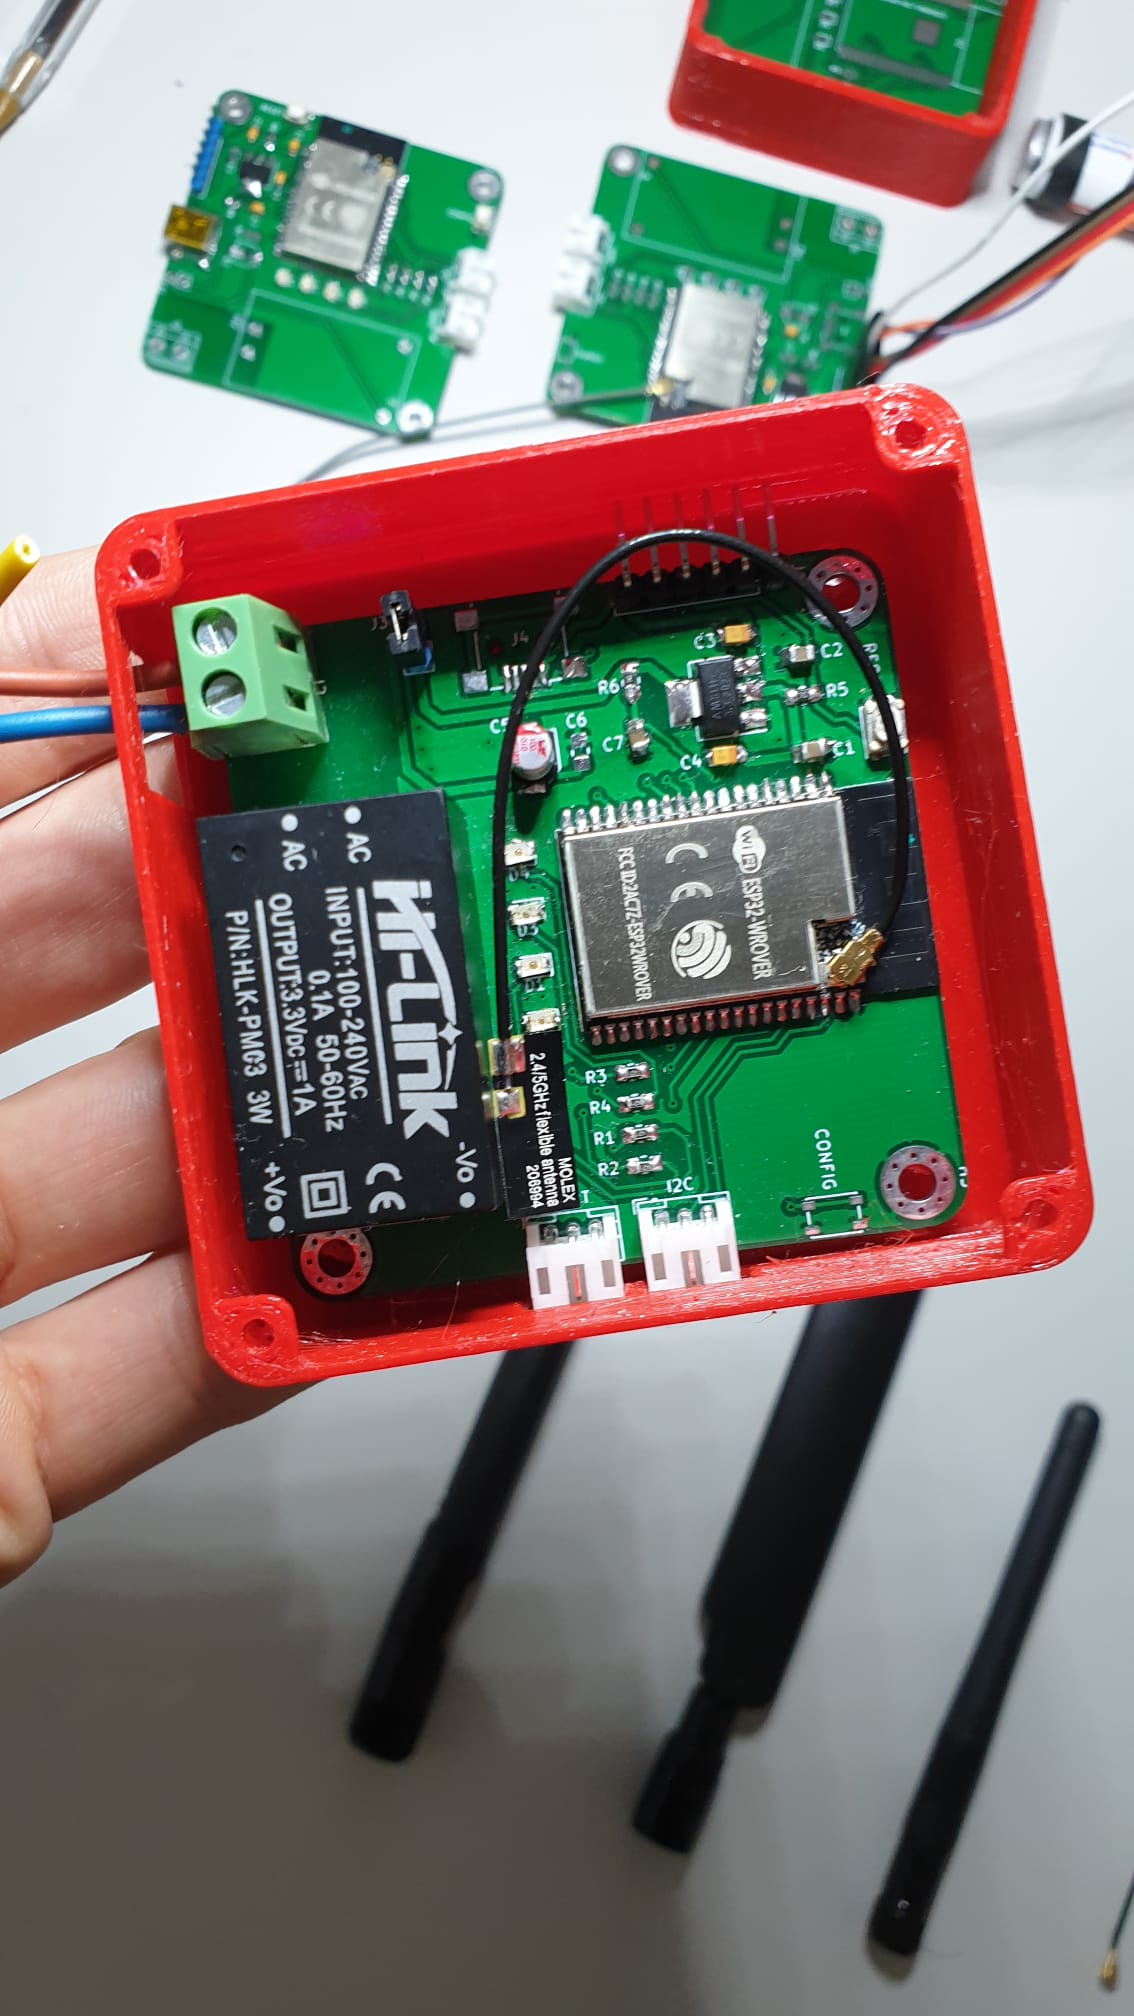
\includegraphics[width=0.4\textwidth]{../3d_antenna.jpeg}
                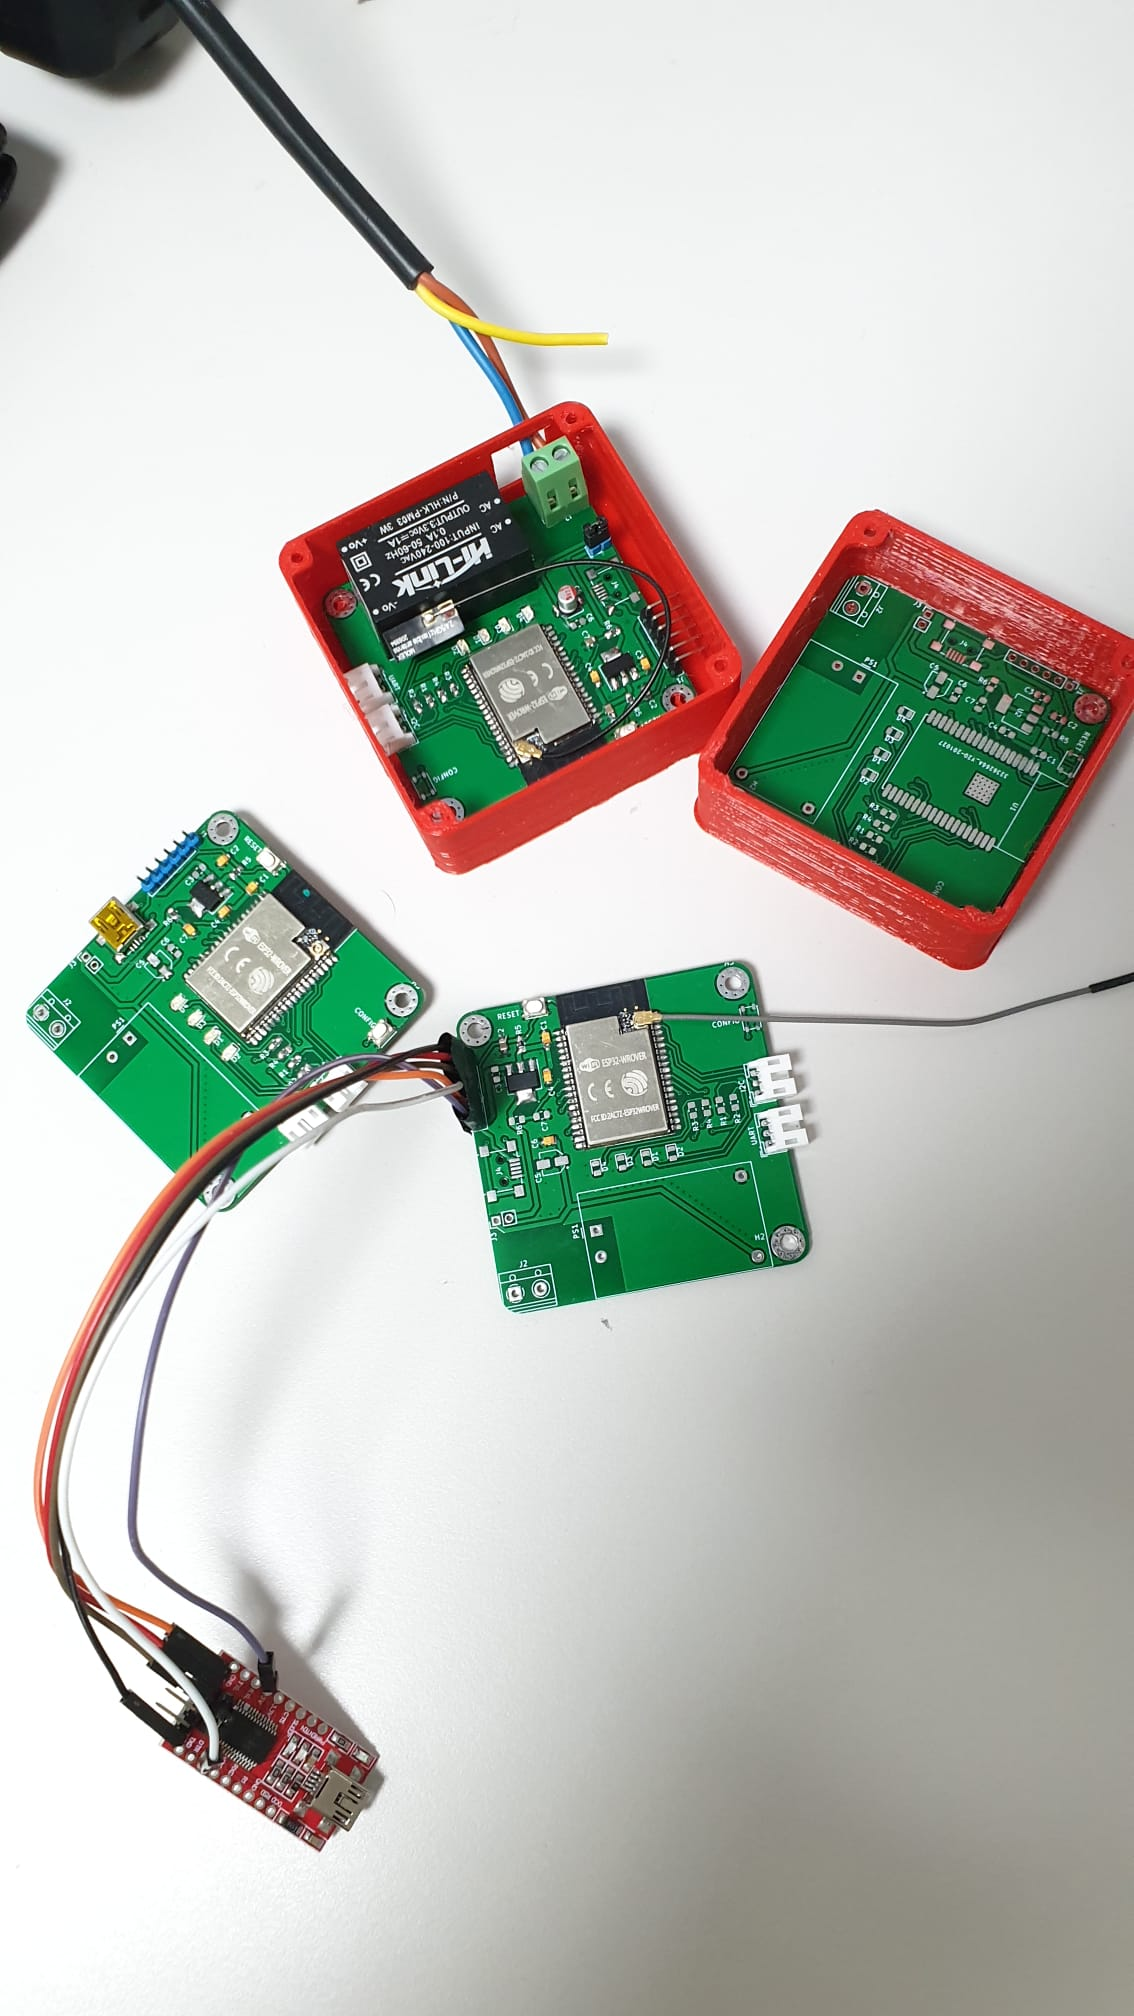
\includegraphics[width=0.51\textwidth]{../real_master_pcb.jpeg}
                \caption{Imágenes reales de la PCB gateway.}
                \label{fig:mesh7}
            \end{figure}    
        \end{center}


    \subsection{Conclusiones}
        Una vez recibidas las PCBs se fueron ensamblando a mano sin mayor incidente que la confusión en la 
        posición de un led que, por supuesto, tras cargar el firmware en la tarjeta, no se iluminó.
        Solucionado el incidente, la versión 1 de las tarjetas fue, por suerte, la definitiva.
\end{document}